\chapter[Tecnologías]{Tecnologías}
\label{Chap2}

\section{Lenguaje de Programación Python}

\subsection{Qué es Python?}
Siendo su primera aparición en el año 1991 por manos de Guido van Rossum, Python es un lenguaje de programación de alto nivel interpretado que prima la legibilidad del código, siendo este a veces nominado como "seudocódigo ejecutable". \cite{dierbach2014python}
\newline
\newline
Python a su vez es un lenguaje multiplataforma, fuertemente tipado, dinámico y multiparadigma, pues soporta programación orientada a objetos, imperativa y funcional. \cite{PyDoc} \cite{borges2014python}

\subsection{Por qué Python?}
La elección de Python sobre otros lenguajes se basa en su sintaxis sencilla y clara que facilita la programación, junto a la gran cantidad de librerías y frameworks potentes de los que dispone para satisfacer las necesidades que presenta este proyecto, como pueden ser la extracción de datos meteorológicos mediante web scraping y la creación de una API.

\newpage

\section{Sistema Operativo Debian}

\subsection{Historia}
Conforme la computación fue tomando terreno tanto en el ámbito comercial como en el escolar, no tener una forma de instalar y configurar los sistemas de una forma rápida sin tener que partir de cero y sin tener que compilar el software necesario manualmente se convirtió en un problema patente entre los usuarios. \cite{krafft2005debian} \cite{hertzog2015debian}
\newline
\newline
En 1993, tras varios intento fallidos por distintas empresas de solucionar el problema, Ian Murdock, por aquel entonces estudiante de la Universidad Purdue, encontró la solución al problema basándose en el reciente proyecto de Linus Torvalds, el kernel Linux. tras el anuncio de Ian para crear un sistema operativo de forma descentralizada en paralelo como es el caso del kernel Linux, docenas de usuarios se unieron para formar el proyecto Debian Linux con la intención de crear un sistema operativo de gran calidad y mantenimiento, publicando en enero de 1994 la primera versión de Debian 0.91. \cite{DebHis}

\subsection{Filosofía}
Debian no intenta seguir ni competir con los lideres del sector, por el contrario, desde sus inicios el proyecto se ha basado en una filosofía centrada en la robustez y estabilidad del sistema guiada por unos estrictos estándares de calidad, actualizándose conforme las necesidades de sus usuarios a la vez que promueve el software gratuito, lo que le ha ayudado a obtener fama entre los usuarios. \cite{DebFil} \cite{pollei2013debian}
\newline
\newline
A su vez, debido al apoyo del software libre, hace uso de múltiples licencias de software como la Licencia Pública General GNU (GPL), licencias artísticas o del tipo BSD, lo cual ha llevado al desarrollo de las Directrices de Software Libre de Debian (DFSG) con el fin de definir la construcción del software libre. \cite{DebFree}
\newpage
Definido por estas licencias, el software libre debe cumplir al menos las que están consideradas la cuatro libertades esenciales: \cite{GnuFS}
\begin{itemize}
	\item Ejecutar el programa como se desee, con cualquier propósito.
	\item Estudiar cómo funciona el programa, y cambiarlo para que haga lo que se desee.
	\item Redistribuir copias para ayudar a otros.
	\item Distribuir copias de sus versiones modificadas a terceros permitiendo ofrecer a toda la comunidad la oportunidad de beneficiarse de las modificaciones.
\end{itemize}

\subsection{Modelo de negocio}
Todo el modelo del proyecto Debian se basa en su Contrato Social respecto a la comunidad de software libre creado en 1997, sobre el cual se estipulan las directrices a seguir para crear y distribuir software libre. \cite{DebCS}
\newline
\newline
No hay que confundir el termino libre, definido dentro de DFSG, con gratuito, pues un programa de software puede ser libre aunque sea de pago. Por el contrario, Debian es un proyecto libre y gratuito.
\newline
\newline
Debian se mantiene gracias a su comunidad, disponiendo más de mil desarrolladores y contribuidores por todo el mundo aportando al proyecto con su tiempo y conocimiento de forma gratuita. Esto, junto a la asistencia de múltiples empresas que dan soporte a Debian dentro del proyecto de socios \cite{DebPP} y el sistema de donaciones \cite{DebDon} usado para hardware, dominios, certificados criptográficos, conferencias, etc han ayudado en el éxito y crecimiento del proyecto dentro de su filosofía.

\subsection{Por qué Debian?}
El mercado está repleto de distintas posibles alternativas a Debian, ya sean de pago, Windows Server OS o Red Hat Enterprise Linux (RHEL), gratuitos, Ubuntu Server y Fedora Server, o incluso en la nube, Amazon Web Services (AWS), Google’s Cloud Platform.
\newline
\newline
Descartando todo sistema de pago, aunque las posibilidades se reducen aun hay múltiples opciones sobre las que elegir, pero son pocas las que ofrecen la misma usabilidad que Debian con sus más de 59000 paquetes en su versión estable o incluso puedes usar las versiones «en pruebas» o «inestable» en caso de querer probar las nuevas funciones antes de su lanzamiento oficial. \cite{DebWhy}
\newline
\newline
Aunque todos los sistemas basados en Linux disponen de las mismas características, siendo software libre y gratuito con soporte multi-usuario, multi-proceso y uso en tiempo real, Debian siendo uno de los sistemas más longevos del mercado a tomado fama entre la competencia por su seguridad y estabilidad. Siendo la base para muchas de las distribuciones más populares contra las que compite, como Ubuntu, Knoppix, PureOS o Tails.
\newline
\newline
Cabe mencionar, que parte de esta seguridad y estabilidad puede llegar a ser un limitante a la hora de elegir Debian como sistema operativo dependiendo de tus necesidades a nivel de uso pues el software compatible igual no es la versión más reciente.
\newline
\newline
Finalmente, una característica distintiva de Debian frente a la competencia gratuita es su compatibilidad con un uso 24/7, pues otras alternativas gratuitas o no dan soporte a esta característica, Fedora Server o, necesitas disponer de una licencia de pago como es el caso de Ubuntu Server mediante Ubuntu Pro.
\newline
\newline
Una vez contado todo esto, puesto que no me afecta negativamente el no disponer de las versiones más recientes de software y necesito de un sistema 24/7 gratuito, parece lógica la elección de Debian como sistema operativo para usar en el servidor.

\newpage

\section{Framework}

\subsection{Qué es un framework?}
Un framework es software que provee una infraestructura básica sobre la que desarrollar tus proyectos, aportando las funcionalidades y estructuras básicas necesarias para este sin la necesidad de programar todo desde cero, ahorrando tiempo de desarrollo y aportando robustez al proyecto. \cite{ghimire2020comparative}
\newline
\newline
Cada framework aportará su propia colección de módulos y paquetes específicos para ayudar en el desarrollo, es por esto que generalmente se clasifican en tres clases distintas según funcionalidades. \cite{WebFra}

\subsubsection{Tipos de frameworks}
\textbf{Full Stack}
\newline
Un framework full-stack es apto tanto para deserrollo back-end como front-end, aportando todas las herramientas posibles que ayuden con el desarrollo gráfico de la interfaz de usuario (UI), gestión de bases de datos, protocolos de seguridad y lógica de negocio entre tantos. Siendo Django un ejemplo de framework full-stack. 
\newline
\newline
\textbf{Micro}
\newline
Los framework micro son ligeros por definición, siendo en cierta medida lo contrario de un framework full-stack, pues aunque los componentes que aportan como puede ser la gestión de bases de datos son los mismos, estos no vienen incluidos de forma nativa. Esto se debe a que buscan aportar flexibilidad y libertad a los desarrolladores para que incluyan unicamente aquellas herramientas que necesiten. 
\newline
\newline
Como se explica en la documentación de Flask, uno de los framework tipo micro más relevante, el 'micro' de microframework significa que el núcleo del framework es simple pero extensible.
\newline
\newline
\textbf{Asíncrono}
\newline
Estos framework están dirigidos por eventos. en vez de hacer un manejo operacional linea a linea de las funciones en la que se van ejecutando una detrás de otra, el código asíncrono no es bloqueante por lo que no se espera que un evento termine para ejecutar el siguiente, ejecutándolo de forma simultanea. Debido a esto un framework asíncrono puede llegar a conseguir un gran rendimiento si se usa en un servidor que lo permita.

\newpage

\subsection{Librería vs Framework}
Aunque ambas ofrecen funcionalidades operacionales, su mayor diferencia radica en la especificidad y complejidad de estas.
\newline
\newline
Las librerías están compuestas por múltiples métodos para un uso especifico sin aportar mucha complejidad, realizando una tarea por función.
\newline
\newline
Por el contrario, como los framework tienen en cuenta las posibles necesidades de tu proyecto, pudiéndose permitir ser aún más específicos, ofreciendo la arquitectura y comportamiento básico de la aplicación, dejando la flexibilidad de desarrollar las funcionalidades necesarias para su funcionamiento, aportando herramientas sobre las que trabajar.

\subsection{Django}

\subsubsection{Qué es Django?}
Djanfo es un framework web de tipo full-stack gratuito y de código abierto para Python. Sigue el principio DRY "Don’t Repeat Yourself" por lo que se enfoca en el menor uso de codigo, el desarrollo rápido y la reutilización de componentes. \cite{DjDF} \cite{alchin2013pro}
\newline
\newline
Hace uso de su auto denominado patrón Modelo-Vista-Template (MVT) \ref{fig:ej1} una variante del conocido Modelo-Vista-Controlador (MVC). \cite{ravindran2015django}
\newline
\begin{figure} [h!]
	\centering
	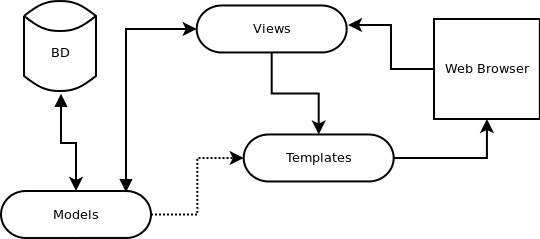
\includegraphics[width=0.7\textwidth]{fig/DjangoMVT.png}
	\caption[Diagrama patrón MVT]{Diagrama patrón MVT}
	\label{fig:ej1}
\end{figure}
\footnotetext{https://docs.hektorprofe.net/django/web-personal/patron-mvt-modelo-vista-template/}
\newline
Para poder trabajar con bases de datos relacionales tales como, Oracle, MySQL y PostgreSQL, Django usa un Mapeador Relacional de Objetos (ORM) permitiendo interactuar con ellas mediante SQL.
\newpage

\subsubsection{Por qué Django?}
Partiendo de que el lenguaje de programación a usar es Python, Django es uno de los frameworks más reputados dirigidos a este lenguaje, teniendo en cuanta su naturaleza gratuita y de código abierto. Siendo usado tanto por la comunidad como por empresas tales como Instagram, Mozilla y Facebook. Aunque no por ello significa que no disponga de poca competencia, siendo TurboGears, web2py, Bottle y Flask de las más notables.
\newline
\newline
El que sea un framework full-stack no va a aportar la flexibilidad, libertad y ligereza que da el uso de un microframework, sobre todo a la hora de agregar únicamente aquellas herramientas que considere necesarias, pero si que atenuará la carga de trabajo que puede suponer un microframework si no se dispone de la experiencia necesaria para usarlo.
\newline
\newline
Otra característica por la que me he decantado por Django, aunque no sea única de él, es su compatibilidad con bases de datos relacionales de forma nativa, cosa que facilitara el uso de estas en el proyecto.

\newpage

\subsection{Scrapy}

\subsubsection{Qué es el Web Scraping?}
Web scraping, también conocido como web extraction o web harvesting, es una técnica de extracción de datos desestructurados de la World Wide web (WWW) y guardarlos de forma estructurada en una base de datos o en un sistema de ficheros en formato XML, JSON o CSV para su posterior recuperación o análisis. Generalmente, los datos web son adquiridos mediante el uso de Hyper-text Transfer Protocol (HTTP) o a través de un navegador web, ya sea de forma manual o automática mediante web crawlers, herramientas diseñadas con este propósito, siendo capaces de convertir páginas web enteras en información bien estructurada.
\newline
\newline
Debido a la gran cantidad de datos que son generados constantemente en la WWW, web scraping es considerado una forma eficiente y poderosa de amasar big data.
\newline
\newline
Web scraping puede ser usado en una gran variedad de entornos, como la recolección de comentarios en redes sociales, listado de la propiedad inmobiliaria o en este caso el monitoreo y comparación de los niveles de los ríos y datos pluviométricos.

\subsubsection{Procedimiento básico en Web Scraping}
El proceso de recolección de datos de internet se puede dividir en dos procesos secuenciales, adquirir los recursos web y, luego, extraer la información deseada.
\newline
\newline
Para realizar este primer paso de adquisición de los recursos, el proceso empieza con los programas de web scraping enviando un request, ya sea mediante GET o POST, a la página web deseada. Una vez el request sea recibido y procesado por la web, esta enviará los recursos solicitados al programa. Después, pasaríamos al segundo paso, en el que analizaríamos los recursos obtenidos y los filtraríamos de tal forma que nos quedásemos únicamente con la información que nos sea necesaria. Finalmente almacenaríamos la información obtenida para su posterior análisis.
\newline
\begin{figure} [h!]
	\centering
	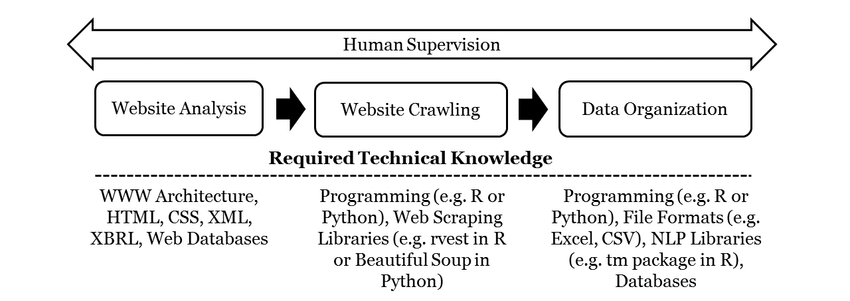
\includegraphics[width=0.7\textwidth]{fig/Web-Scraping-Adapted-from-Krotov-and-Tennyson-2018.png}
	\caption[Web Scraping (Krotov y Tennyson 2018)]{Web Scraping}
	\label{fig:ej2}
\end{figure}
\footnotetext{\url{https://www.researchgate.net/figure/Web-Scraping-Adapted-from-Krotov-and-Tennyson-2018_fig1_324907302}}
\newline

\subsubsection{Qué es Scrapy?}
Scrapy es un framework asíncrono para web crawling y web scraping gratuito y de código abierto. Por defecto proporciona todas las herramientas necesarias para realizar la tarea de extracción, procesado y estructurado de los datos adquiridos, ademas de dar la opción de extender funcionalidades en caso necesario, haciéndolo extremadamente versátil.
\newline
\newline
Pensado para navegar entre webs y extraer información de forma estructurada de ellas, Scrapy es usado para múltiples propósitos, por ejemplo, el minado de datos o la monitorización y análisis de datos.

\subsubsection{Por qué Scrapy?}
A la hora de buscar herramientas para web scraping en Python obtuve tres alternativas principales, BeautifulSoup, Selenium y Scrapy.
\newline
\newline
La primera es una librería de parseo de HTML y XML, que, aunque podría haberme servido para mi propósito inicialmente, a la larga su sencillez hubiera sido más un problema que una ayuda.
\newline
\newline
La segunda por el contrario, no es una herramienta para hacer web scraping como tal y se centra en la automatización de la navegación web como entorno de pruebas. Debido a esto, no es una herramienta que haya usado para el web scraping, pero si que ha sido usada junto con Scrapy para navegar entre webs 
y sacar los datos de estas.
\newline
\newline
Scrapy fue elegida gracias a la flexibilidad y versatilidad que proporciona a la hora de trabajar, pudiendo crear proyectos sencillos en cuestión de minutos con las herramientas base proporcionadas o investigar como trabajar con estas herramientas y crear proyectos complejos que satisfagan tus necesidades de la manera que desees. Esto implica que la curva de aprendizaje de Scrapy sea mayor que la que puede tener BeautifulSoup sobre todo al inicio, llegando a parecer abrumador. A su vez, Scrapy tiene el mejor rendimiento entre las tres.
\newline
\newline
Finalmente, cabe mencionar que Scrapy no dispone de rotación de IP, renderizado JavaScript, ni geolocalización como pueden tener las alternativas de pago, cosa que no es un impedimento para llevar a cabo el proyecto. 